\documentclass{beamer}
\usepackage{amsfonts,amsmath,oldgerm}
\usepackage{ragged2e}

\usetheme{sintef}

\newcommand{\testcolor}[1]{\colorbox{#1}{\textcolor{#1}{test}}~\texttt{#1}}

\usefonttheme[onlymath]{serif}

\titlebackground*{assets/background}

\newcommand{\hrefcol}[2]{\textcolor{cyan}{\href{#1}{#2}}}

\title{Aula 01 - Computação em nuvem PT-1}
\subtitle{2023.1 - LESA 6 -  Laboratório de Escalabilidade de Sistemas}
\course{Tecnologia em Análise e Desenvolvimento de Sistemas}
\author{\href{mailto:luiz.quirino@ifsp.edu.br}{Luiz \textbf{Quirino}}}
\IDnumber{luiz.quirino@ifsp.edu.br}



\begin{document}
\maketitle
\footlinecolor{maincolor}

\section{Conceitos e objetivos}

\begin{frame}[fragile]{Objetivos desta aula}\justifying
      \begin{itemize}
            \item Entender o conceito da computação em nuvem;
            \item Conhecer os modelos de computação em nuvem e seus principais serviços;
            \item Entender como as empresas estão usando a computação em nuvem - quando usar e quando não usar;
            \item Saber analisar custos e benefícios.
      \end{itemize}
\end{frame}

\begin{frame}[fragile]{O que é computação em nuvem?}\justifying
      Parece uma pergunta simples, mas as aparências enganam.
\end{frame}



\section{Introdução}
\begin{frame}[fragile]{O que é computação em nuvem?}\justifying
      \begin{itemize}
            \item Seria outro nome para aplicações hospedadas em Data Centers?
            \item Seria um sinônimo para virtualização?
            \item Seria apenas uma jogada de marketing para definir uma nova cara em uma antiga tecnologia?
      \end{itemize}
      Em 1961, o professor John McCarthy sugeriu que a tecnologia de computação compartilhada, poderia levar a um futuro onde a computação se transformaria em um modelo de negócio do tipo utilitário.
\end{frame}
\begin{frame}[fragile]{O que é computação em nuvem?}\justifying
      Em 1968, Licklider, então diretor da Advanced Research Projects Agency (ARPA), descreveu a sua visão de computação como sendo “um conjunto de funções e serviços disponíveis na rede, onde os usuários podem contratar uma base regular e outros que os usuários invocam quando necessitarem deles”.
\end{frame}
\begin{frame}[fragile]{O que é computação em nuvem?}\justifying
      \begin{itemize}
            \item "É uma solução completa na qual todos os recursos de computação (hardware, software, rede, armazenamento, etc.) são fornecidos rapidamente a usuários à medida que a demanda exigir".
            \item "Um serviço usado e tarifado sob demanda".
      \end{itemize}
\end{frame}


\begin{frame}[fragile]{O instituto Gartner e a computação em nuvem}\justifying
      \begin{center}
            \Large{O instituto Gartner definiu cinco atributos que considera essenciais para caracterizar a computação em nuvem.}
      \end{center}
\end{frame}


\begin{frame}[fragile]{O instituto Gartner e a computação em nuvem}\justifying
      \begin{itemize}
            \item Oferta de recursos (infraestrutura e aplicações) como serviços;
            \item Elasticidade e escala adequadas à demanda do cliente;
            \item Compartilhamento de recursos entre um grande número de usuários;
            \item Medição e pagamento de acordo com o uso do serviço;
            \item Utilização de protocolos e tecnologias da internet para acesso aos recursos na nuvem (pública ou privada).
      \end{itemize}
\end{frame}

\section{Por que optar por computação em nuvem?}
\begin{frame}[fragile]{Os serviços da computação em nuvem:}\justifying
      Possuem a capacidade de ter seus recursos aumentados ou reduzidos, conforme a demanda.
\end{frame}


\begin{frame}[fragile]{Os serviços são controláveis, para assegurar:}\justifying
      \begin{itemize}
            \item Alta disponibilidade
            \item Segurança
            \item Qualidade
            \item Elasticidade
      \end{itemize}
\end{frame}
\begin{frame}[fragile]{Pode reduzir custos associados ao fornecimento de serviços de TI:}\justifying
      \begin{itemize}
            \item Infraestrutura de hardware
            \item Infraestrutura de software:  banco de dados, editores de texto, planilhas, editores de imagem etc.
            \item Pessoal especializado
            \item Consumo de energia
            \item Atualização de hardware e software
            \item Obter recursos somente quando são necessários e pagando somente quando são usados
      \end{itemize}
\end{frame}
\begin{frame}[fragile]{Por que computação em nuvem?}\justifying
      \begin{itemize}
            \item Capacidade de combinar muitas tecnologias existentes:
            \begin{itemize}
                  \item SOA (Service-Oriented Architecture ) - Arquitetura orientada a serviços;
                  \item Virtualização;
                  \item Computação autônoma: desenvolvimento de sistemas computacionais capazes de autogerenciamento e adaptação a mudanças imprevisíveis.
            \end{itemize}
      \end{itemize}
\end{frame}

\section{Anatomia de uma nuvem}
\begin{frame}[fragile]{Os três principais componentes da computação em nuvem}\justifying
      Podem ser representados pelas seguintes camadas:
      \begin{itemize}
            \item Software como serviço SaaS - (Software as a Service)
            \item Plataforma como serviço PaaS - (Platform as a Service)
            \item Infraestrutura como serviço IaaS – (Infrastructure as a Service)
      \end{itemize}
\end{frame}
\begin{frame}[fragile]{Software como serviço - SaaS (Software as a Service)}\justifying
      \begin{itemize}
            \item Essa camada é, possivelmente, a mais familiar para usuários da web comuns;
            \item Hospeda aplicativos que se encaixam no modelo SaaS;
            \item Estes aplicativos podem ser gratuitos ou não;
      \end{itemize}
\end{frame}
\begin{frame}[fragile]{Software como serviço - SaaS (Software as a Service)}\justifying
      Exemplos:
      \begin{itemize}
            \item GMail
            \item Yahoo Mail
            \item Exchange Online
            \item Google Docs
            \item Google Calendar
            \item Office 365
      \end{itemize}
\end{frame}
\begin{frame}[fragile]{Software como serviço - SaaS (Software as a Service)}\justifying
      Muitos aplicativos na camada Saas são direcionados à comunidade corporativa:
      \begin{itemize}
            \item Processamento de folha de pagamento;
            \item Gerenciamento de recursos humanos;
            \item Colaboração;
            \item Gerenciamento de relacionamento com o cliente;
            \item Gerenciamento de parceiros de negócios.
      \end{itemize}
\end{frame}
\begin{frame}[fragile]{Exemplos:}\justifying
      \begin{itemize}
            \item IBM Lotus Live (reuniões on-line)
            \item IBM Lotus Sametime (comunicações sociais)
            \item Salesforce (CRM)
            \item Microsoft Exchange Online (e-mail)
      \end{itemize}
\end{frame}
\begin{frame}[fragile]{Software como serviço - SaaS (Software as a Service)}\justifying
      \begin{itemize}
            \item Os aplicativos fornecidos através do modelo SaaS beneficiam consumidores aliviando-os da instalação e manutenção de software;
            \item Podem ser usados através de modelos de licenciamento que suportam pagamento para conceitos de uso.
      \end{itemize}
\end{frame}
\begin{frame}[fragile]{Software como serviço - SaaS (Software as a Service) - Vantagens}\justifying
      \begin{itemize}
            \item Maior tempo para validar e melhorar a produtividade quando comparado aos longos ciclos de aplicação e taxa de falha de software empresarial;
            \item Custo de licenciamento muito inferiores;
            \item Maior economia na manutenção e atualização do software;
            \item Fornecedores de SaaS possuem auditoria de segurança meticulosas.
      \end{itemize}
\end{frame}
\begin{frame}[fragile]{Software como serviço - SaaS (Software as a Service) - Desvantagens}\justifying
      \begin{itemize}
            \item O cliente deve se adaptar às parametrizações do software;
            \item Criar aplicações para serem entregues a milhares de clientes de forma eficiente, por intermédio da internet, é um trabalho árduo;
            \item Personalização complexa da aplicação para atender necessidades específicas;
            \item Depende da banda para entrega eficiente do produto;
      \end{itemize}
\end{frame}

\begin{frame}[fragile]{Plataforma como serviço - PaaS - (Platform as a Service)}\justifying
      Essa é a camada na qual vemos a infraestrutura do aplicativo emergir como um conjunto de serviços.
\end{frame}
\begin{frame}[fragile]{São serviços que suportam a execução dos aplicativos da camada SaaS}\justifying
      \begin{itemize}
            \item IBM® WebSphere® Application Server;
            \item Amazon Web Services (AWS);
            \item Google App Engine;
            \item Microsoft Windows Azure;
            \item Microsoft SQL Azure.
      \end{itemize}
\end{frame}
\begin{frame}[fragile]{Plataforma como serviço - PaaS - (Platform as a Service)}\justifying
      Estes serviços possibilitam que os clientes tenham certeza de que seus aplicativos estejam equipados para atender as necessidades de usuários, fornecendo a infraestrutura do aplicativo com base na demanda de uso.
\end{frame}
\begin{frame}[fragile]{Infraestrutura como serviço - IaaS (Infrastructure as a Service)}\justifying
      Camada responsável pela infraestrutura de hardware (elementos físicos) oferecidos como serviços provisionados a consumidores
      \begin{itemize}
            \item Servidores;
            \item Dispositivos de rede;
            \item Discos;
            \item Memória;
      \end{itemize}
\end{frame}
\begin{frame}[fragile]{Infraestrutura como serviço - IaaS (Infrastructure as a Service)}\justifying
      Os serviços de infraestrutura abordam o problema de equipar de forma apropriada o data center, assegurando o poder de computação quando necessário. O uso das técnicas de virtualização, empregadas nesta camada, propicia maior economia de custos decorrentes da utilização mais eficiente dos recursos de hardware.
\end{frame}



\begin{frame}[fragile]{Infraestrutura como serviço - IaaS (Infrastructure as a Service)}\justifying
      Com a elasticidade da virtualização, é possível adequar o hardware à demanda.
      \begin{itemize}
            \item Nuvens públicas;
            \item Nuvens privadas;
            \item Nuvens Híbridas.
      \end{itemize}
\end{frame}
\begin{frame}[fragile]{Infraestrutura como serviço - IaaS (Infrastructure as a Service) \\ Nuvens públicas}\justifying
      \begin{itemize}
            \item São serviços em nuvem fornecidos por terceiros;
            \item Existem além do firewall da empresa;
            \item São completamente hospedadas e gerenciadas pelo provedor da nuvem.
      \end{itemize}
\end{frame}
\begin{frame}[fragile]{Infraestrutura como serviço - IaaS (Infrastructure as a Service) \\ Nuvens públicas (Vantagens)}\justifying
      \begin{itemize}
            \item Tentam oferecer elementos de TI sem problemas (software, infraestrutura de aplicativo ou infraestrutura física);
            \item O provedor da nuvem assume as responsabilidades de instalação, gerenciamento, fornecimento e manutenção;
            \item Os clientes são cobrados somente pelos recursos usados, portanto, a subutilização é eliminada.
      \end{itemize}
\end{frame}
\begin{frame}[fragile]{Infraestrutura como serviço - IaaS (Infrastructure as a Service) \\ Nuvens públicas (Desvantagens)}\justifying
      \begin{itemize}
            \item As opções de configuração são mais restritas;
            \item O consumidor tem pouco controle sobre a infraestrutura;
            \item Os processos que requerem forte segurança e conformidade reguladora nem sempre são uma boa adequação para nuvens públicas.
      \end{itemize}
\end{frame}
\begin{frame}[fragile]{Infraestrutura como serviço - IaaS (Infrastructure as a Service) \\ Nuvens públicas (Desvantagens)}\justifying
      \begin{itemize}
            \item As opções de configuração são mais restritas;
            \item O consumidor tem pouco controle sobre a infraestrutura;
            \item Os processos que requerem forte segurança e conformidade reguladora nem sempre são uma boa adequação para nuvens públicas.
      \end{itemize}
\end{frame}
\begin{frame}[fragile]{Infraestrutura como serviço - IaaS (Infrastructure as a Service) \\ Nuvens privadas}\justifying
      \begin{itemize}
            \item Os serviços são fornecidos dentro da empresa;
            \item Estas nuvens existem dentro do firewall da empresa e são gerenciadas pela empresa;
            \item A empresa é responsável por configurar e manter a nuvem.
      \end{itemize}
\end{frame}
\begin{frame}[fragile]{Infraestrutura como serviço - IaaS (Infrastructure as a Service) \\ Nuvens privadas (Vantagens)}\justifying
      \begin{itemize}
            \item Total controle sobre os serviços prestados;
            \item Tranquilidade com a segurança e regulação das informações.
      \end{itemize}
\end{frame}
\begin{frame}[fragile]{Infraestrutura como serviço - IaaS (Infrastructure as a Service) \\ Nuvens privadas (Desvantagens)}\justifying
      \begin{itemize}
            \item Alto custo em infraestrutura de hardware;
            \item Exige a presença de pessoal especializado;
            \item Tempo elevado de implantação;
            \item Alocação de espaço físico e segurança;
            \item As responsabilidades de instalação, gerenciamento, fornecimento e manutenção ficam por conta do cliente;
      \end{itemize}
\end{frame}
\begin{frame}[fragile]{Infraestrutura como serviço - IaaS (Infrastructure as a Service) \\ Nuvens híbridas}\justifying
      \begin{itemize}
            \item Uma combinação de nuvens públicas e privadas;
            \item Usa serviços que estão no espaço público e no privado;
            \item Responsabilidade compartilhada entre a empresa e o provedor de nuvem pública;
      \end{itemize}
\end{frame}
\begin{frame}[fragile]{Infraestrutura como serviço - IaaS (Infrastructure as a Service) \\ Nuvens híbridas (Vantagens)}\justifying
      \begin{itemize}
            \item Maior flexibilidade para a implantação de serviços, conforme as necessidades;
            \item Se bem construída, pode atender processos seguros e críticos para a missão.
      \end{itemize}
\end{frame}
\begin{frame}[fragile]{Infraestrutura como serviço - IaaS (Infrastructure as a Service) \\ Nuvens híbridas (Desvantagens)}\justifying
      \begin{itemize}
            \item Dificuldade de criar e controlar de forma efetiva tal solução;
            \item As interações entre componentes privados e públicos podem tornar sua implantação mais complicada;
            \item Como o modelo é relativamente novo, sua implementação pode se tornar mais relutante.
      \end{itemize}
\end{frame}

\section{Decisões estratégicas}
\begin{frame}[fragile]{Resumão}\justifying
      O uso da computação em nuvem depende de diversos fatores:
      \begin{itemize}
            \item Taxa custo/benefício;
            \item Velocidade de transferência;
            \item Capacidade a ser usada;
            \item Se os dados estão organizados;
            \item Administração da empresa e sua estrutura de TI.
      \end{itemize}
\end{frame}

\begin{frame}[fragile]{Quando EVITAR a computação em nuvem}\justifying
      Dados altamente confidenciais: a privacidade da informação
      pode estar mais comprometida em uma nuvem pública.
      O SLA (Service Level Agreement - Acordo de nível de serviço)
      deve ser bem analisado.
\end{frame}
\begin{frame}[fragile]{Quando EVITAR a computação em nuvem}\justifying
      Assuntos legislativos: existem leis que permitem ao governo
      ter acesso aos dados públicos com maior facilidade do que
      dados privados.
 \end{frame}
 \begin{frame}[fragile]{Quando EVITAR a computação em nuvem}\justifying
      Preocupações geopolíticas: dados de uma empresa
      brasileira podem estar hospedados nos Estados Unidos e
      poderão estar sujeito às leis do país hospedeiro.
  \end{frame}
  \begin{frame}[fragile]{Quando EVITAR a computação em nuvem}\justifying
      Falta de necessidade: Nuvem não é modismo - é
      necessidade. “Se não está quebrado - não conserte”.
  \end{frame}
  \begin{frame}[fragile]{Quando EVITAR a computação em nuvem}\justifying
      Demanda e quantidade de dados: aplicações de altíssima
      demanda devem sofrer um estudo apurado de
      custo/benefício.
  \end{frame}
  \begin{frame}[fragile]{O que os empresários temem na nuvem}\justifying
      Uma recente pesquisa realizada pelo IDC com 244 executivos de TI revelou as seguintes preocupações (em porcentagem):
      
      \begin{itemize}
          \item Reversão do processo
          \item Fornecedores
          \item Disponibilidade
          \item Desempenho
          \item Segurança
      \end{itemize}
      
      \end{frame}
      


















\begin{frame}[fragile]{Imagem do dia}
      \framesubtitle{Computação em nuvem}
	\begin{figure}[H]
		\centerline{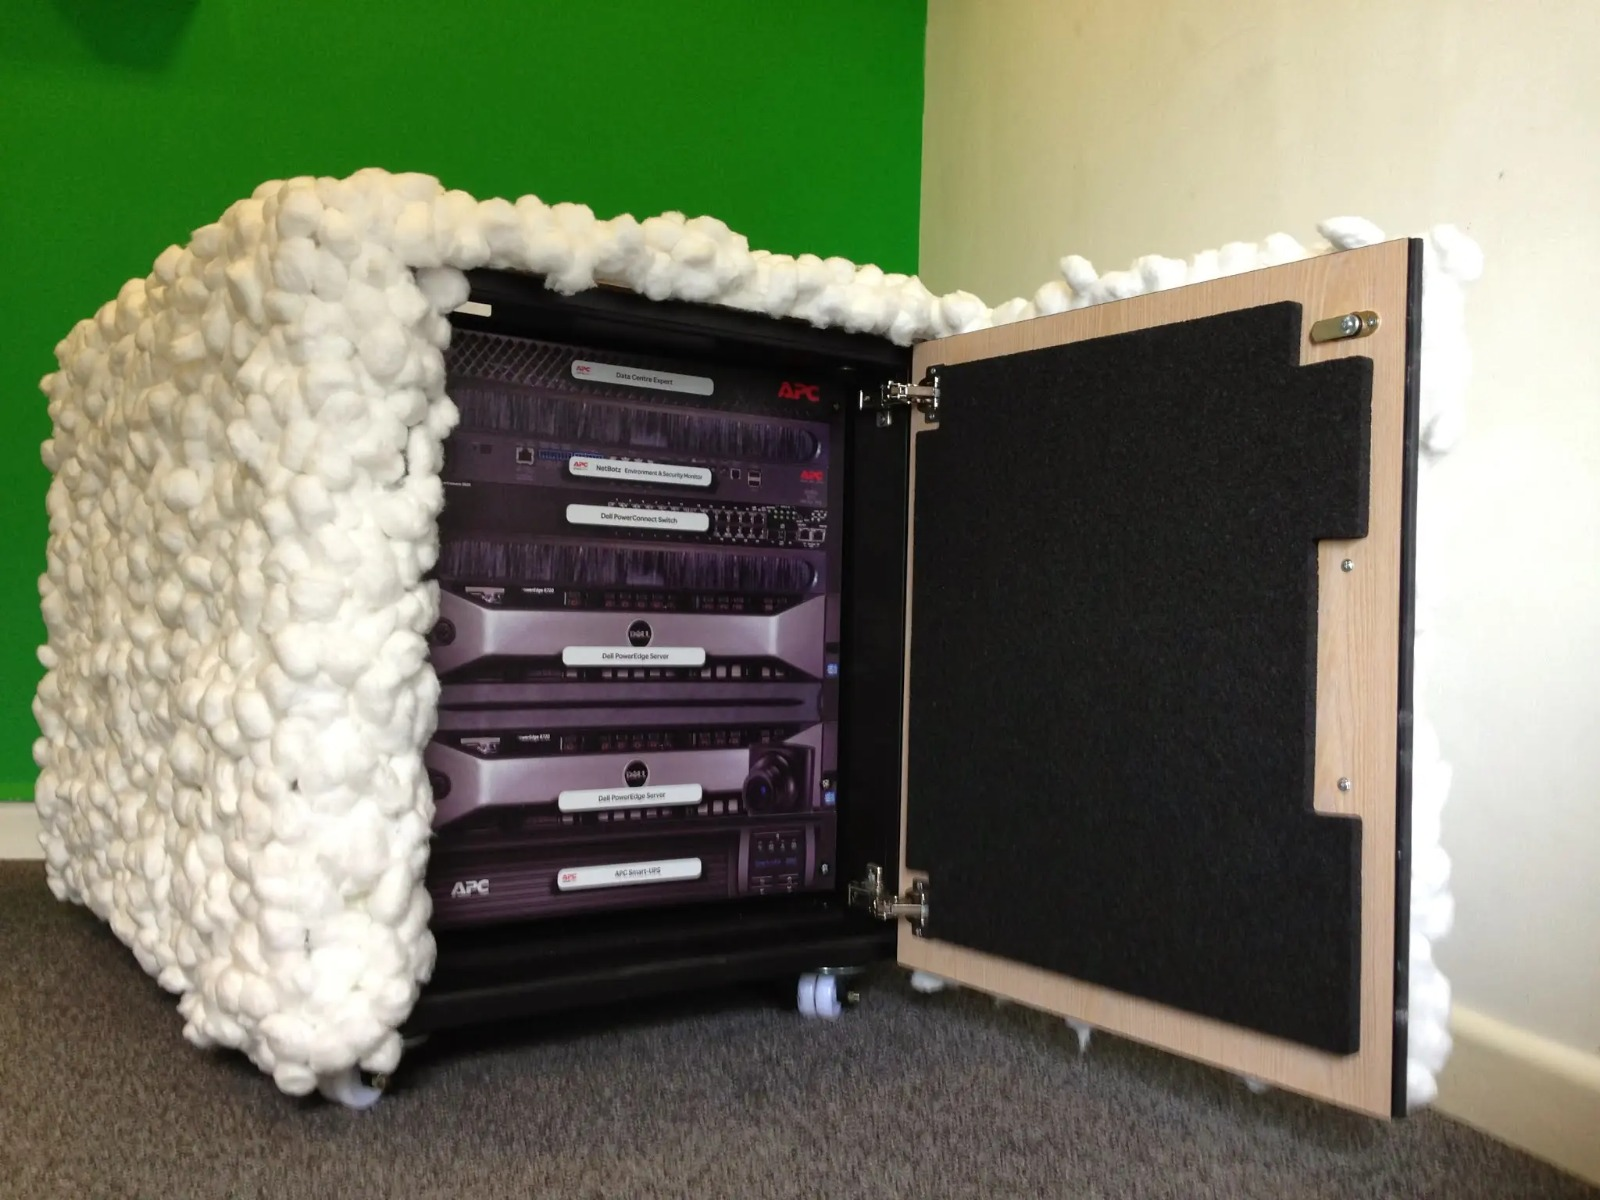
\includegraphics[width=0.5\textwidth]{assets/imagem-do-dia/nuvem-computador.jpeg}}

	\end{figure}
\end{frame}
\footlinecolor{}

\backmatter
\end{document}
